\section{Resultados}

Los resultados de la prueba descrita se muestran en la tabla \ref{tab:Resultados}.

\begin{table}[ht]
	\centering
	\begin{tabular}{|c|c|c|c|c|}
		\hline
		\textbf{$L_1$ (cm)} & \textbf{$L_2$ (cm)} & \textbf{Tiempo total (s)} & \textbf{Error máximo (cm)} & \textbf{Tamaño (MB)} \\
		\hline
		3 & 4 & 70 & 0.68 & 3.05 \\
		7 & 8 & 100 & 0.66 & 3.08 \\
		10.5 & 12 & 110 & 0.66 & 3.12 \\
		14.5 & 16 & 115 & 0.66 & 3.17 \\
		18 & 21 & 120 & 0.66 & 3.26 \\
		\hline
	\end{tabular}
	\caption{Resultados}
	\label{tab:Resultados}
\end{table}

Se pudo notar que el tiempo de la clusterización es de alrededor de 2 minutos. Esto es por la cantidad de posturas generadas para determinar la más cercana a una posición en particular; si la base rota en 360°, y las articulaciones rotan 90°, entonces:

\begin{equation}
	360 \cdot 90 \cdot 90 = 2,916,000
\end{equation}

Lo que quiere decir que se generan 2,916,000 posturas. Esto es un valor relativamente alto, que puede ser reducido si se varían en ángulos de 2° en las articulaciones; por el enfoque que hemos dado al modelo, sabemos que la distancia de un punto con coordenadas enteras a otro es, por la distancia euclidiana, de 0.707 cm, de modo que la precisión no disminuye significativamente si disminuimos la cantidad de ángulos que pueden ser generados por cada articulación. Sin embargo, la cantidad de posiciones alcanzables puede verse reducida, debido a que algunas posiciones solo podrían ser alcanzadas por alguna postura en particular que no se consideró para la clusterización. Este valor aumentará exponencialmente conforme aumente la cantidad de grados de libertad de acuerdo con lo siguiente:

\begin{equation}
	P = 360 \cdot 90^n
\end{equation}

Donde n es la cantidad de grados de libertad.

También puede notarse que el tamaño conjunto de los archivos de clusterización no crece exponencialmente al variar la longitud de las articulaciones; se mantiene cercana a 3,2 MB, lo cual es un tamaño relativamente pequeño en comparación con el almacenamiento de la Raspberry Pi utilizado para este proyecto, de 16 GB. Si se aumentan los grados de libertad, cada archivo de clusterización guarda 1 byte más de información.

Un resultado a destacar es que el sistema requiere un tiempo constante de ejecución para determinar la cinemática inversa; cuando se tiene un punto $P(x,y,z)$ de entrada, se toman los 8 puntos vecinos y se determina el más cercano, y luego se toman los ángulos del archivo correspondiente a esa posición, lo que implica una lectura de 4 bytes. Si se ignoran las operaciones de lectura de los datos, que se ejecutan en un tiempo mayor que si se leyeran de la memoria RAM, existen a lo más 12 operaciones para determinar la cinemática inversa, lo que demuestra que el sistema tiene un tiempo de respuesta muy rápido, de acuerdo con la capacidad de la Raspberry Pi.

El brazo de prueba a ser controlado se muestra en la Figura \ref{fig:brazoSEDPC}.

\begin{figure}[htb]
	\centering
	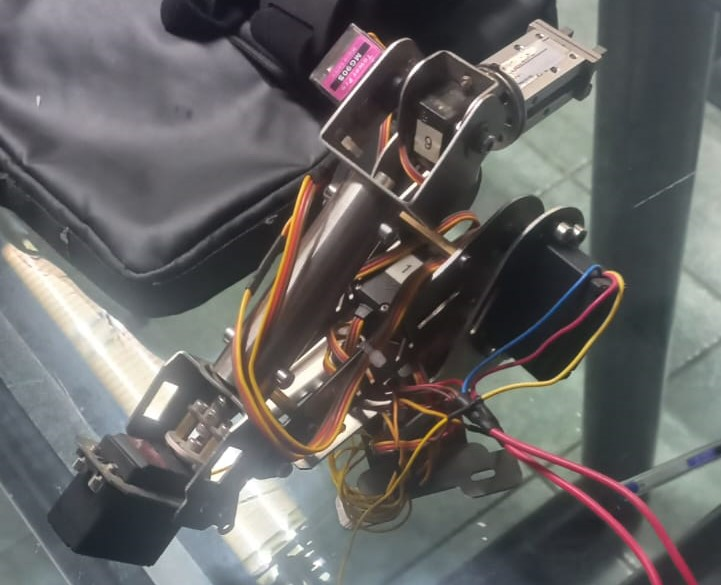
\includegraphics[scale=0.5]{brazoSEDPC.jpg}
	\caption{Brazo robótico proporcionado por SEDPC para la demostración}
	\label{fig:brazoSEDPC}
\end{figure}